\chapter[Resultados]{Resultados}

A partir do estudo e pesquisa realizado até o momento determinamos o que utilizar no conjunto do sistema, levantando um perfil que a equipe acredita ser a mais viável em termos de interação, custo-benefício, tempo, conhecimento técnico e outros fatores importantes para o projeto. Será desenvolvido um kit com capacidade de ser acoplado em diversas cadeiras de rodas afim de facilitar a mobilidade elétrica em cadeiras manuais. Os resultados levantados estão disposto no decorrer do capítulo.

\section{Estrutura}

Com a utilização do programa CATIA V5 3D foi estruturado o sistema eletrônico acoplado à cadeira de rodas, \ref{fig:vista_isometrica_traseira}. Visando três preceitos básicos: comodidade, acessibilidade e conforto.

\begin{figure}[!htb]
\centering
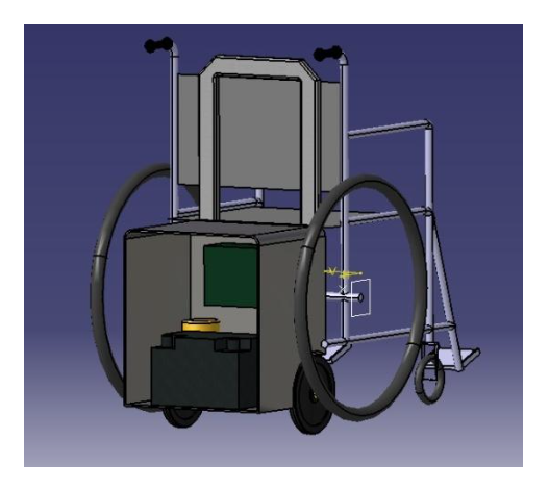
\includegraphics[keepaspectratio=true,scale=0.4]{figuras/estrutura/vista_isometrica_traseira}
\caption{Vista Isométrica Traseira}
\label{fig:vista_isometrica_traseira}
\end{figure}

O objetivo do projeto é desenvolver uma estrutura de fácil conexão e resistente. O produto proposto, ver figura \ref{fig:traseira}, \ref{fig:sistema}, \ref{fig:lateral} e \ref{fig:superior},deve-se acoplar a qualquer cadeira de rodas.

Foi pensado em um dispositivo no formato de uma mala para que seja de fácil conexão, uso e manuseio.

\begin{figure}[!htb]
\centering
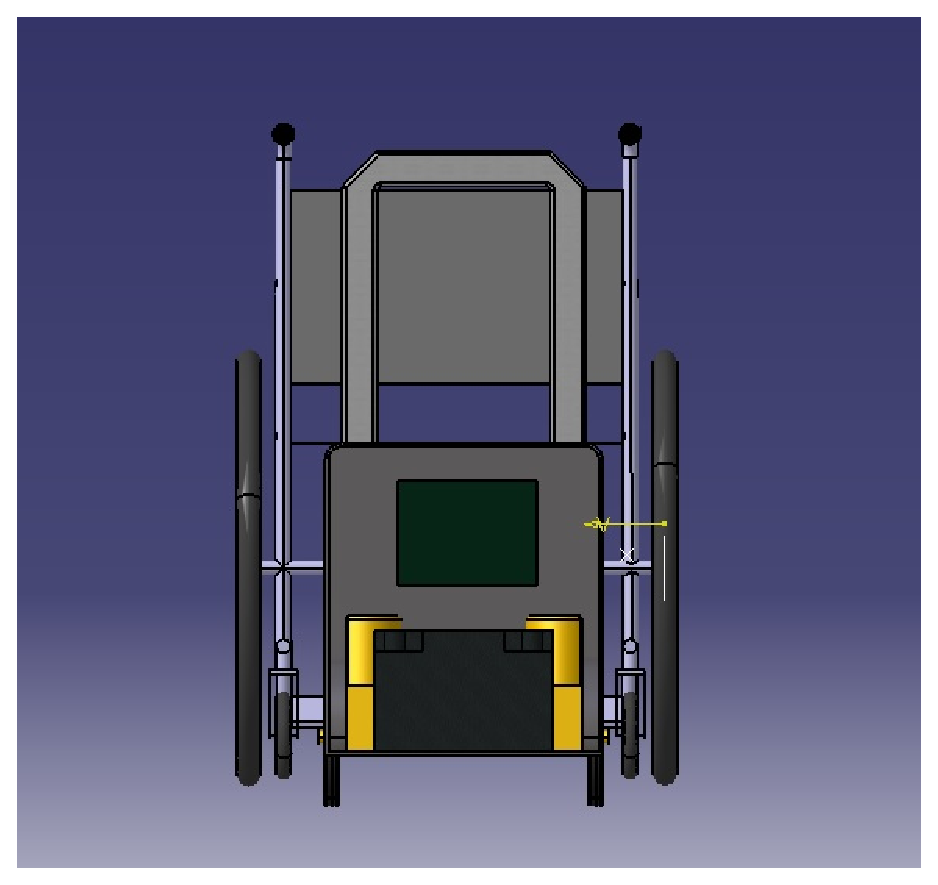
\includegraphics[keepaspectratio=true,scale=0.4]{figuras/estrutura/vista_traseira}
\caption{Vista Traseira}
\label{fig:traseira}
\end{figure}

A forma como a mala será acoplada a cadeira usa como base as hastes da mala e as hastes verticais aonde as manoplas utilizadas para empurrar manualmente a cadeira são fixadas. Tendo em vista que são rígidas e normatizadas pela NBR 9050 as hastes verticais da cadeira tem a distancia e espessura já definidas, o que facilita o desenvolvimento de um produto que possa ser usado em qualquer cadeira de rodas que esteja dentro dos padrões impostos pela norma.

\begin{figure}[!htb]
\centering
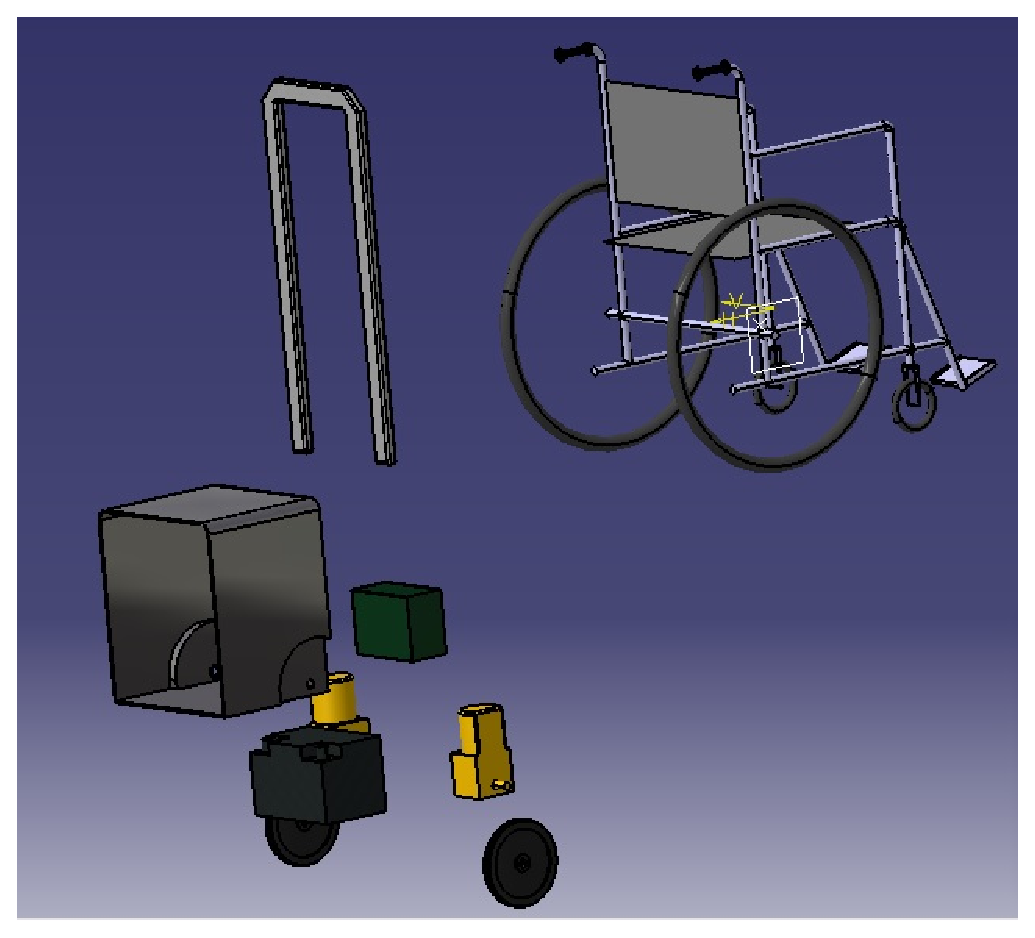
\includegraphics[keepaspectratio=true,scale=0.4]{figuras/estrutura/explode}
\caption{Visão do Sistema}
\label{fig:sistema}
\end{figure}

Cada roda possuirá um motor próprio para que seja possível rotaciona-lás em sentidos opostos, por exemplo, quando for necessário fazer manobras em que a rotação deve ocorre em torno do eixo do próprio cadeirante, movimento muito comum para manobrar uma cadeira de rodas. Assim o cadeirante se sentira confortável e não terá grandes dificuldades quando for manobrar a cadeira, já que a lógica de controle será a mesma usada quando se propulsiona manualmente a cadeira.

\begin{figure}[!htb]
\centering
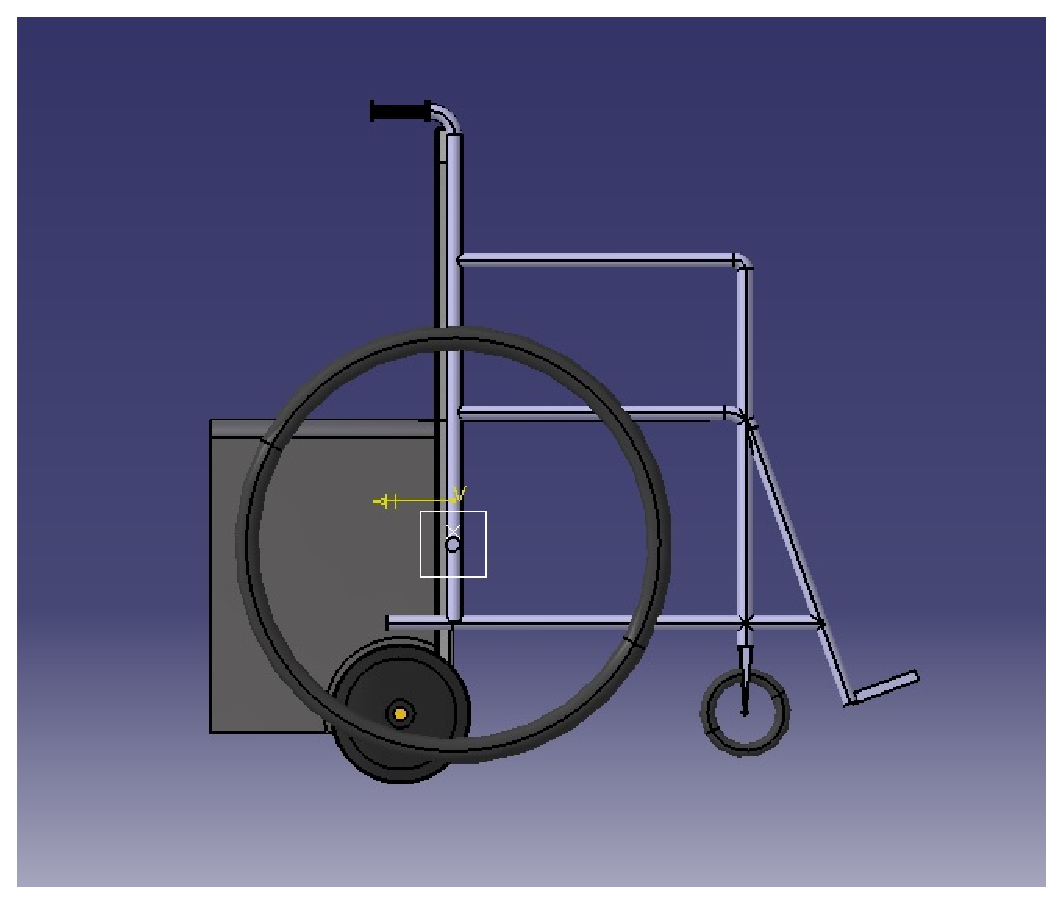
\includegraphics[keepaspectratio=true,scale=0.4]{figuras/estrutura/vista_lateral_cadeira}
\caption{Imagem Lateral}
\label{fig:lateral}
\end{figure}

Como pode se notar nas figuras, o sistema de propulsão devera empurrar a cadeira de rodas, pois assim podemos aproximar o máximo possível o eixo da roda que ira gerar o movimento ao eixo da maior roda da cadeira, o que diminui a quantidade de torque necessário para movimentar o conjunto, fazendo com que o consumo de energia diminua e possibilite o uso de um motor de menor potencia, que diminuirá o custo do produto final.

\begin{figure}[!htb]
\centering
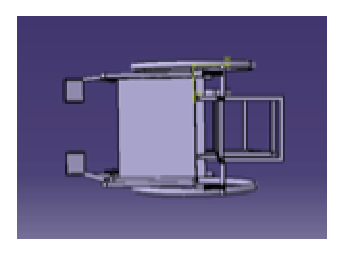
\includegraphics[keepaspectratio=true,scale=0.4]{figuras/estrutura/vista_superior}
\caption{Imagem Superior}
\label{fig:superior}
\end{figure}

\subsection{Protótipo}

A partir do policloreto de vinila, usualmente conhecido como PVC, foi feita uma estrutura de teste para encaixar na parte de trás da cadeira de rodas, com o intuito de buscar a melhor regulação to tamanho da estrutura. O protótipo em questão foi feito para se chegar o mais próximo de um modelo ideal capaz de se acoplar as cadeiras regulamentadas pela NBR 9050.

O protótipo é uma estrutura retangular com uma alça de regulação de largura, seguido de dois “joelhos” em PVC para o acoplamento das rodinhas e da haste, dois encaixes com três saídas para regulação da barra de encaixe superior da cadeira. Há quatro furos na barra de regulação de largura, a qual serve para se adequar ao tipo de cadeira de rodas sendo utilizada, vide figura para mais detalhes \ref{fig:acoplamento}.

\begin{figure}[!htb]
\centering
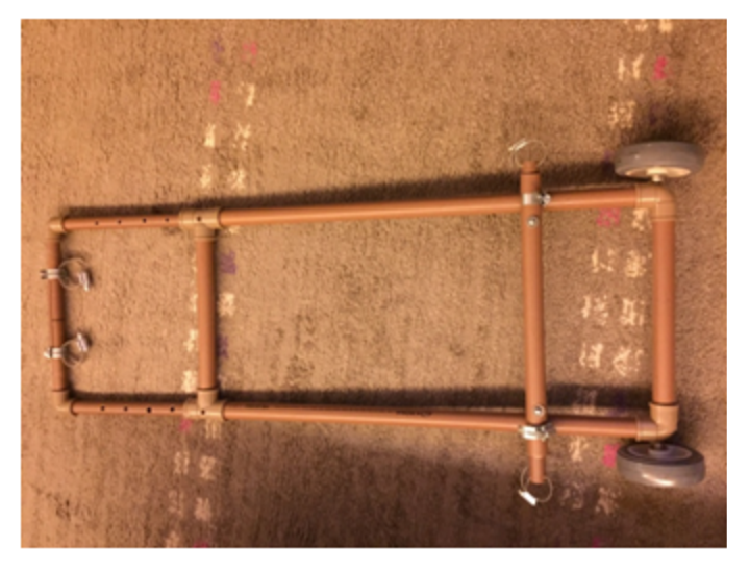
\includegraphics[keepaspectratio=true,scale=0.7]{figuras/resultados/acoplamento}
\caption{Estrutura de acoplamento}
\label{fig:acoplamento}
\end{figure}

No protótipo foram usadas oito braçadeiras circulares de curso infinito, as quais se acoplam na cadeira de rodas dando rigidez a estrutura, dessas oito braçadeiras, duas na parte inferior se acoplam na parte de baixo da cadeira, outras duas se acoplam na parte superior. A figura \ref{fig:acop_bracadeira} ilustra o sistema de acoplamento estrutura/cadeira.

\begin{figure}[!htb]
\centering
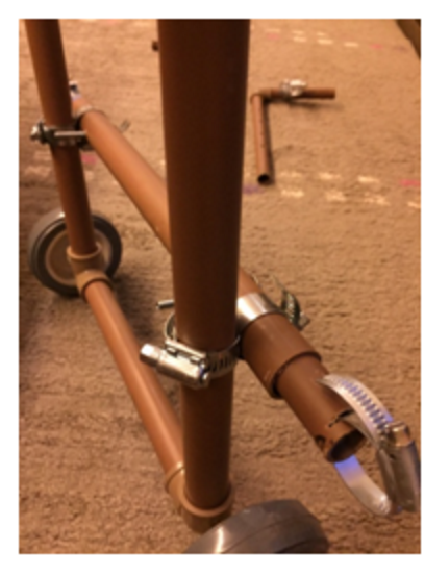
\includegraphics[keepaspectratio=true,scale=0.7]{figuras/resultados/acop_bracadeira}
\caption{Sistema de acoplamento com braçadeira}
\label{fig:acop_bracadeira}
\end{figure}

Na parte da estrutura mostrada na figura \ref{fig:acop_bracadeira} existem dois “joelhos” que ligam as rodinhas com o as barras de PVC, além de uma barra em paralelo com a barra das rodinhas, capaz de variar em altura e largura para se adequar ao tamanho da cadeira utilizada, e  duas braçadeiras nas pontas das barras que irão se acoplar a cadeira de rodas.

\begin{figure}[!htb]
\centering
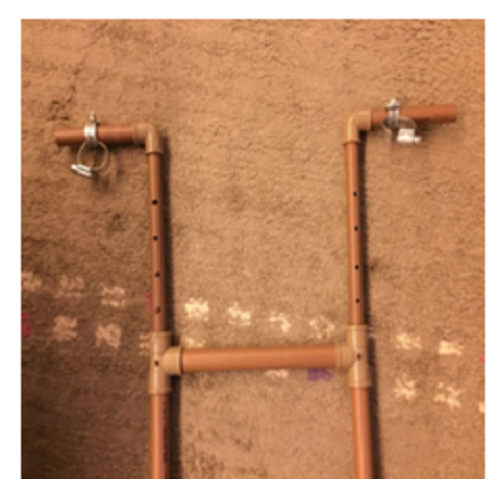
\includegraphics[keepaspectratio=true,scale=0.7]{figuras/resultados/superior_estrutura}
\caption{Parte superior da estrutura}
\label{fig:superior_estrutura}
\end{figure}

A figura \ref{fig:superior_estrutura} representa a parte superior da estrutura, ela contem dois “joelhos” capazes de ligar as duas alças com as duas barras de sustentação da estrutura. Há dois “T” com furo que ligam três barras de cada lado, eles tem a função de regular a altura com o seis furos nas barras de movimentação. Na alça estão duas braçadeiras livres, que se ligam na parte superior da cadeira de rodas, assim como a parte superior já descrita.

Os componentes utilizados para se fazer este modelo são descritos:
\begin{itemize}
  \item Oito braçadeiras circulares de curso infinito;
  \item Quarto “joelhos” de 90$^\circ$;
  \item Dois “T”;
  \item Duas rodas;
  \item Barras de PVC com diâmetros de 20mm e 25mm;
  \item Quatro parafusos;
  \item Oito arruelas;
  \item Quatro porcas.
\end{itemize}

O protótipo apresentado na figura \ref{fig:estr_prototipo} foi capaz de mostrar como funcionará o sistema, e todo encaixe necessário para não ocorrer folga e desconforto ao cadeirante. Esta estrutura se assemelha com as medidas do sistema original, mudando apenas o material da execução e do funcionamento. Obteve-se excelentes resultados testando tal protótipo em dois modelos de cadeira de rodas.

\begin{figure}[!htb]
\centering
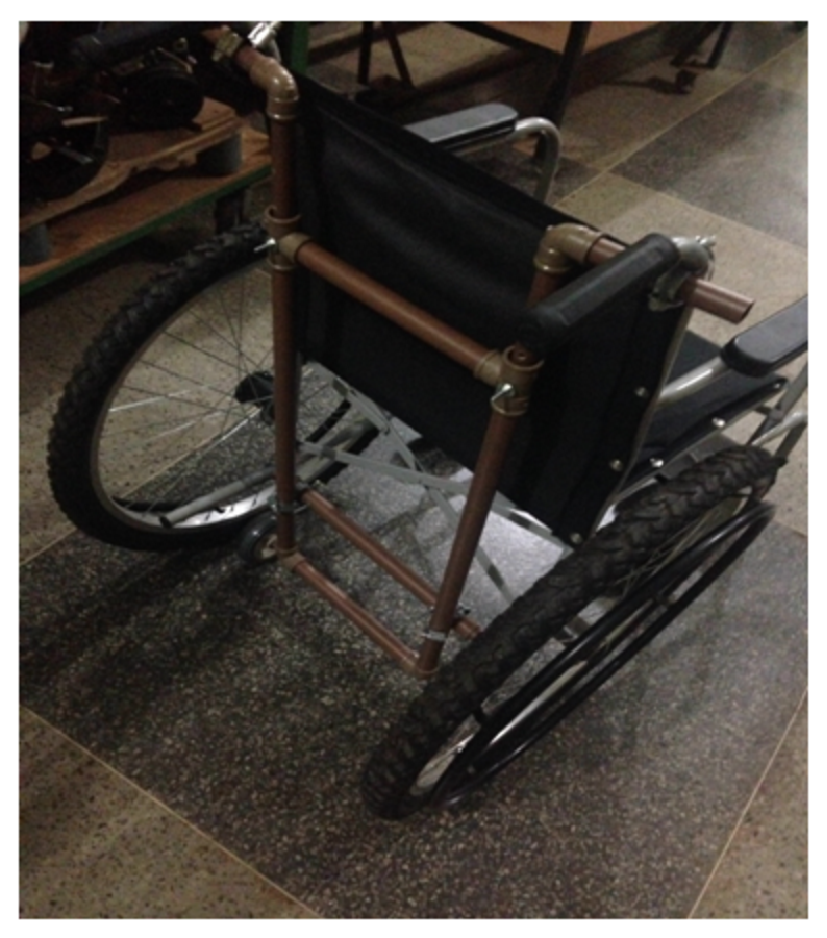
\includegraphics[keepaspectratio=true,scale=0.7]{figuras/resultados/estr_prototipo}
\caption{Estrutura acoplada a cadeira}
\label{fig:estr_prototipo}
\end{figure}

\section{Power-Train}

\subsection{Moto-redutor}

Será utilizado no projeto o motor de corrente contínua. A escolha foi feita pois esse tipo de motor é muito utilizado em projetos que necessitam de velocidades variáveis, eles também apresentam uma região de torque e potência constante e são simples de realizar a aceleração e a desaceleração \cite{manual_bateria_unipower}.

Após uma vasta pesquisa no mercado de motores e redutores, optou-se por comprar dois moto-redutores feitos pela empresa MKS Redutores de São Paulo. O motor com redutor escolhido para o projeto foi o MR com motor GPB que possui as seguintes especificações:

\begin{itemize}
  \item Potência de 305 a 350 W;
  \item 12 ou 24 Vcc;
  \item Rotação de entrada de 2500 rpm;
  \item Reduções de 1:10 até 1:60.
\end{itemize}

Especificações a serem atendidas:

\begin{itemize}
  \item Velocidade máxima de 10 km/h;
  \item 12 Volts corrente contínua;
  \item Peso da bateria 15 kg;
  \item Peso da cadeira (valor aproximado) 15kg;
  \item Peso total estimado: 150 Kg;
  \item Redução de pelo menos 1:10.
\end{itemize}

\subsection{Bateria}

A bateria de chumbo-ácido é muito utilizada hoje em dia em diferentes áreas, como automóveis, sistemas de fornecimento de energia elétrica ininterrupta (no-breaks) e cadeiras de rodas elétricas. Desprezando-se o problema do peso e considerando as observações feitas anteriormente no capítulo \ref{cap:fundamentacao_teorica}, a bateria de chumbo-ácido selada foi a escolhida para o projeto, considerando ainda o seu fácil acesso no mercado e baixo custo.

\subsubsection{Autonomia}

Segundo a literatura, cadeiras de rodas elétricas trabalham com motores de corrente contínua entre 250 W a 300 W de potência. Para este projeto se decidiu utilizar motores de 300W. Há diversas maneiras de chegar neste valor, como por distribuição de forças, por balanço de energia, por forças em um plano inclinado, entre outras. Decidiu-se fazer uma estimativa da potência necessária através do balanço de energia.
A energia fornecida pelo motor deve ser igual à energia cinética da cadeira. Sendo a massa máxima que a cadeira de rodas aguenta de 150 kg e considerando que cadeiras de rodas elétricas chegam até 10 km/h, tem-se:

\begin{equation}
Em = \frac{m*V^2*\epsilon}{2}
\end{equation}

Onde $Em$ é a energia fornecida pelo motor, $m$ é a massa de 150 kg e $V$ é a velocidade em metros por segundo. Aqui estimou-se perdas do motor de pelo menos 20\%, sendo assim, $\epsilon$ é igual a 1,20. Assim, a energia necessária para mover a cadeira é de 694 J, a potência é portanto 694 W.

Ao utilizar dois motores de 300 W, a potência total entregue ao sistema seria de 600 W. Rearranjando a equação para encontrar o valor da velocidade, e atribuindo 80\% de eficiência no acoplamento das rodas com o eixo do motor, temos:

\begin{equation}
Em = 0.8*\sqrt{\frac{600*2}{m*\epsilon}}
\end{equation}

Assim, a estimativa da velocidade máxima que a cadeira deve obter será de pelo menos 7.44 km/h, uma velocidade razoável para este tipo de sistema. Sabe-se que a velocidade angular é dada pela divisão da velocidade linear pelo raio:

\begin{equation}
\omega = \frac{V}{r}
\end{equation}

Logo, utilizando a velocidade estimada acima, a velocidade angular obtida é de 20.6 rad/s ou aproximadamente 197 rpm. Considerando as especificações do motor comprado: velocidade angular nominal de 2500 rpm e potência de 305 W, teria de ser feita uma redução de pelo menos 1:10, onde a velocidade angular de saída do redutor seria de 250 rpm. Sendo o torque a divisão da potência pela velocidade angular, o torque gerado é de 29 Nm (Newtons-metro).

Para atender dois motores de 305 W, será conectada uma bateria de carro de chumbo-ácido selado de 12 V (U) e capacidade de 60Ah (I*$\Delta$t), tem-se que a energia $E$ gerada pela bateria é de:

\begin{equation}
E = (I*\Delta t)*U = (60Ah)*12 = 720Wh
\end{equation}

Desta forma, considerando a potência consumida pelos dispositivos eletrônicos de controle desprezível, tem-se que a autonomia da bateria seria de pouco mais de uma hora:

\begin{equation}
\Delta t = \frac{720 Wh}{610 W} = 1.18 h = 1 hora e 10 minutos
\end{equation}

\section{Controle}

 Na Figura \ref{fig:esquema_controle} foi feita uma proposta de construção do kit mostrando a sua estrutura de controle. Em verde claro tem-se um componente que talvez seja somente integrado ao sistema. Esses blocos foram resultado dos estudos teóricos e de discursões da equipe. Em verde escuro, sistemas que serão efetivamente projetados e construídos e em azul, componentes que não serão construídos mas farão parte do kit de automação.

\begin{figure}[!htb]
\centering
  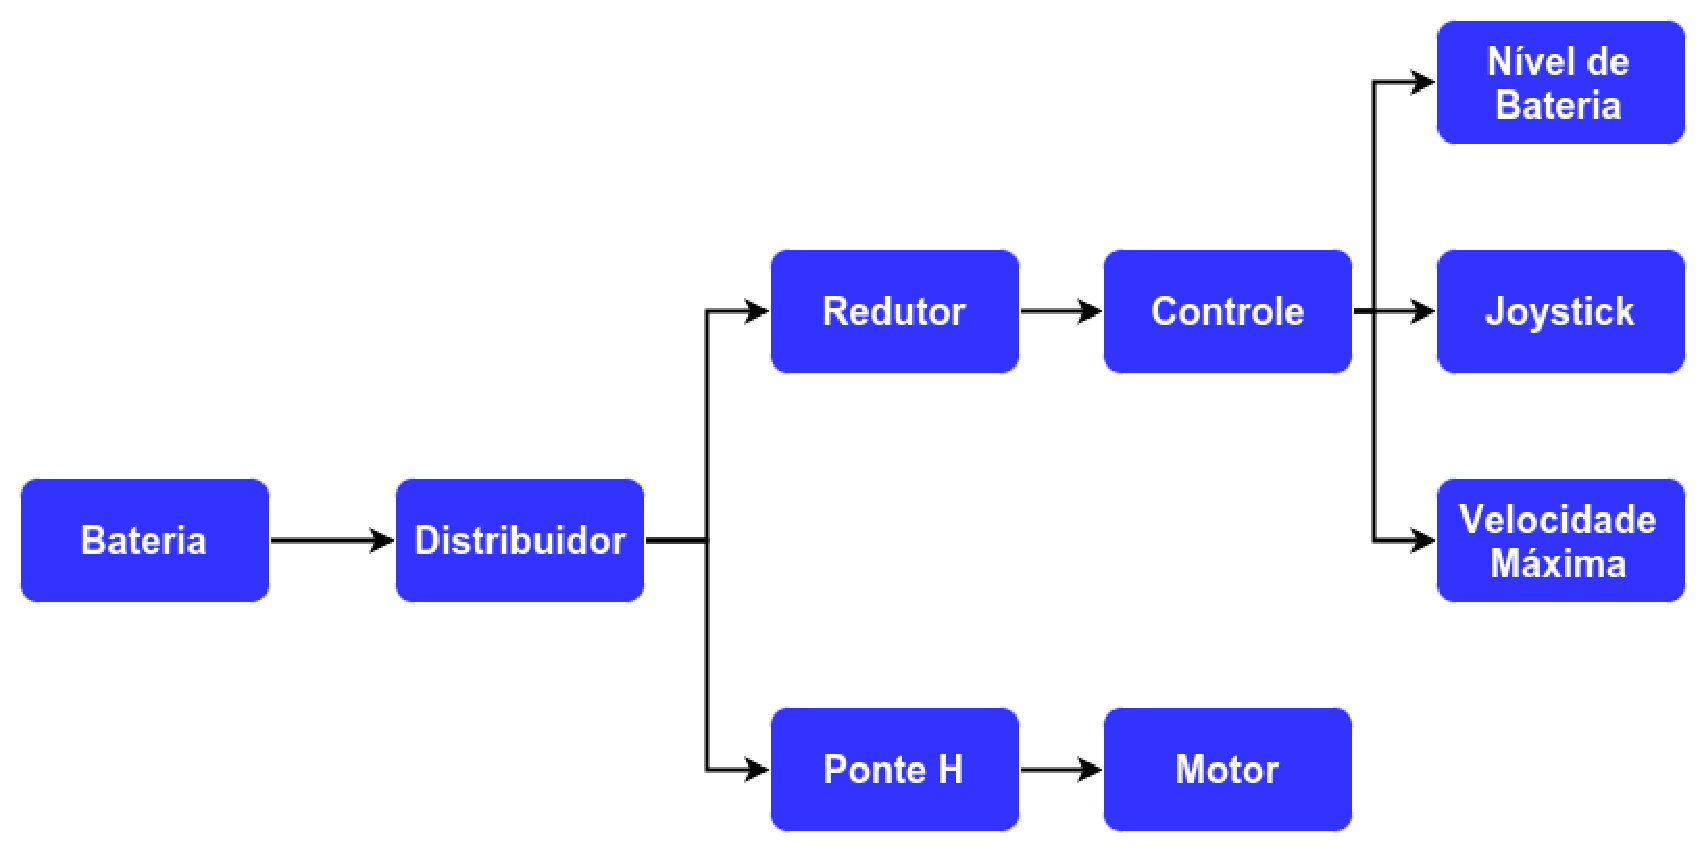
\includegraphics[keepaspectratio=true,scale=0.5]{figuras/resultados/esquema_controle}
\caption{Esquemático de funcionamento geral da cadeira de rodas automatizada}
\label{fig:esquema_controle}
\end{figure}

Para o kit de automação da cadeira de rodas, será utilizada a ponte H para o controle dos motores. Um algoritmo de controle PWM usando o Raspeberry Pi que deve responder aos comandos do usuário como direção, aceleração, frenagem, entre outros que serão posteriormente levantados. Tem-se ainda o Distribuidor, uma placa para facilitar a alimentação do sistema, e o Regulador, para alimentar o Controlador e periféricos.

O sistema vai ser projetado de forma que não seja necessário retirar a bateria para essa ser carregada, o carregador será construído comprado, considerando que o tempo disponível para o desenvolvimento do projeto é relativamente curto.

\subsection{Joystick}

Para as cadeiras de rodas automatizadas essa é uma solução comum de controle para as mesmas, tendo em vista que é relativamente simples de ser acoplado uma vez que se entenda seu funcionamento básico. Para o projeto em questão essa foi uma das alternativas encontradas. No qual o joystick seria acoplado ao braço da cadeira, ou em uma posição que o usuário se sinta mais ergonomicamente confortável. Este acoplamento deve ser simples para favorecer a característica de portabilidade do projeto como um todo.

Nesta iteração foram feitos alguns testes para utilização do joystick, porém ainda não voltado para uso do usuário.

Os testes realizados foram feito como testes de utilização do conjunto motores-ponte H-Raspberry Pi-MSPs.

\subsection{Arquitetura}

Com base no entendimento de como as informações foram entendidas, e na formulação dos diagramas de ideias, foi formulada uma arquitetura inicial para o software de controle do produto.

\begin{figure}[!htb]
\centering
  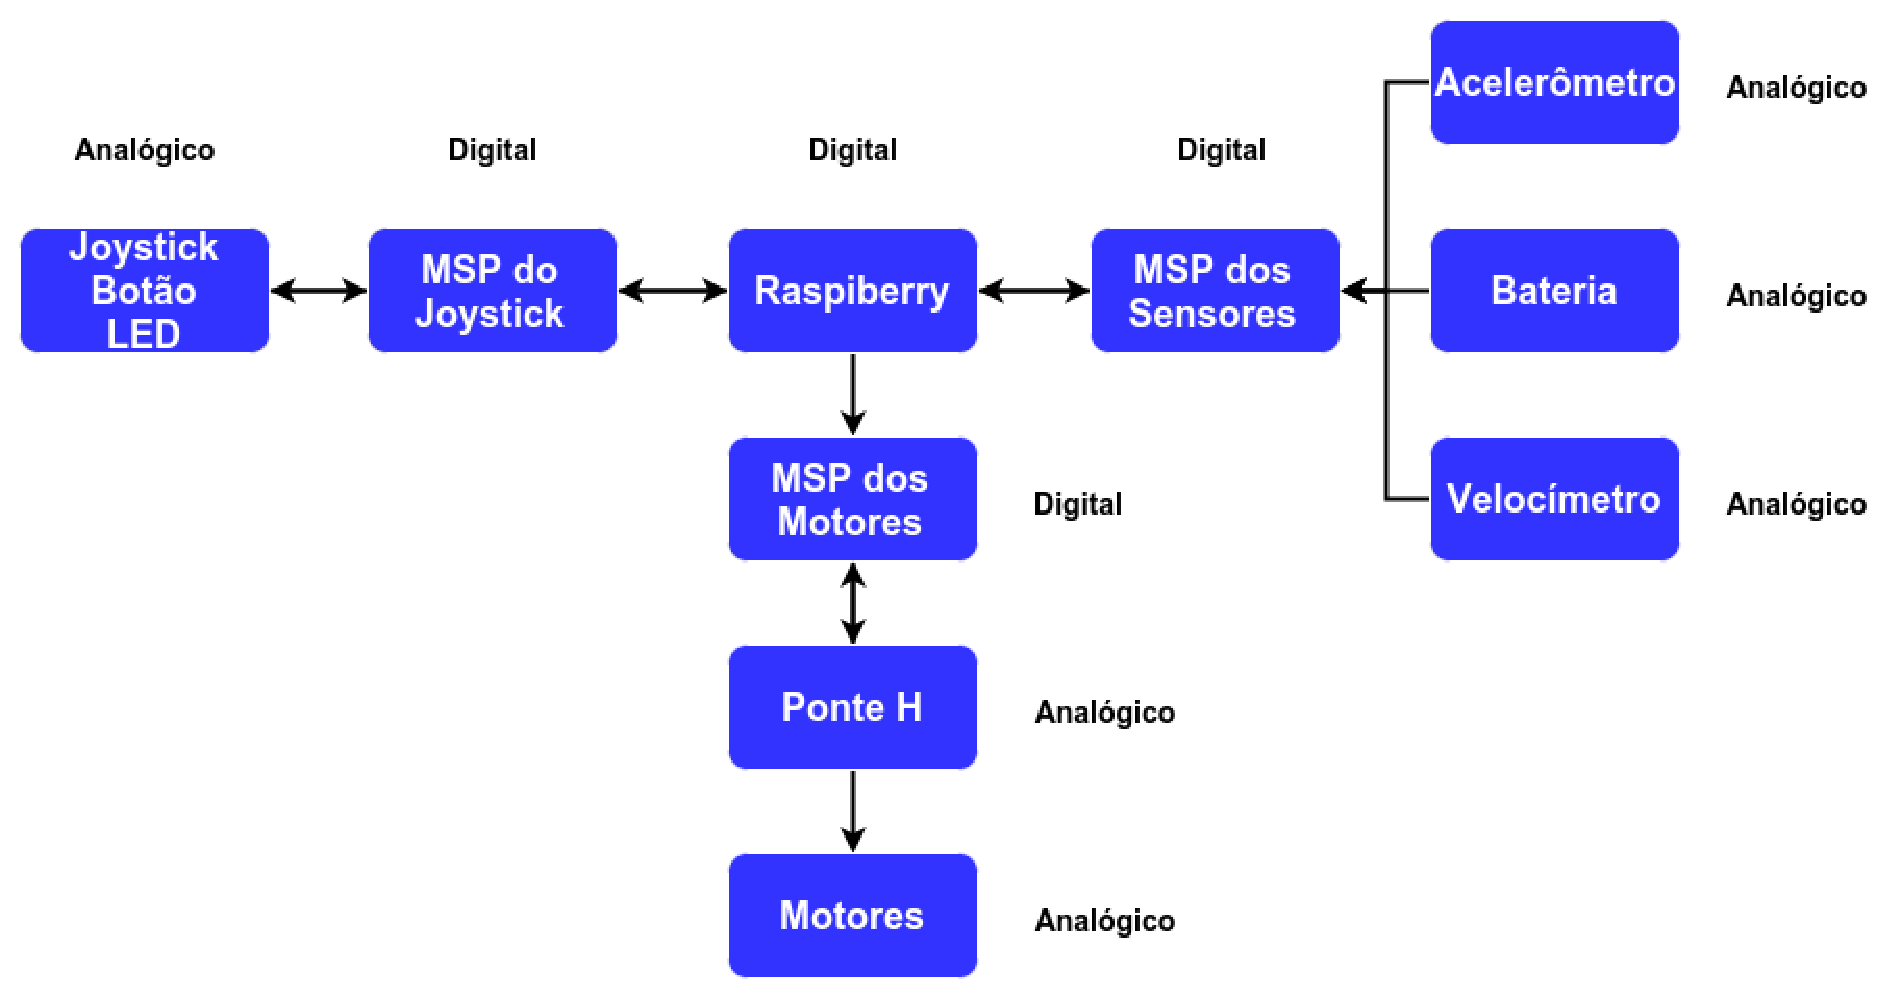
\includegraphics[keepaspectratio=true,scale=0.5]{figuras/resultados/arquitetura}
\caption{Arquitetura}
\label{fig:arquitetura}
\end{figure}

Esta arquitetura pode ser entendida na figura \ref{fig:arquitetura}. Esta figura ilustra a ideia de como a arquitetura se comporta. Imaginando o fluxo da informação, conforme o uso do usuário temos:

\begin{enumerate}
  \item Usuário envia a informação via "Joystick" com os comandos relativos as direções pretendidas. O "Joystick" possui 2 potênciometros que funcionam enviando a informações que variam de 0 a 255.
  \item Esta informação será captada por um MSP, convertendo esse sinal analógico para digital e enviando-o para o Raspberry Pi.
  \item O envio desta informação é recebido, via interrupção, do MSP no Raspberry  Pi. O envio da informação é feito via UART. (esta interrupção recebe a informação através de uma nova thread)
  \item O Raspberry Pi irá tratar esta informação das direções que o usuário pretende seguir, em intensidade e direção que os motores devem agir. E então a informação é passada para o MSP que controla a Ponte-H. O envio da  informação é feito via UART.
  \item O MSP que controla a Ponte-H recebe a informação e a traduz em 2 pulsos de onda quadrada, que tem como intuito enviar cada um destes pulsos para uma Ponte-H diferente.
  \item A Ponte-H controla os motores.
\end{enumerate}

A parte relacionada ao sensoriamento ainda não foi completamente estabelecida, mas pretende-se adicionar sensores ou algum outro mecanismo capaz de aferir o nível de bateria, velocidade e nível de inclinação da cadeira.

Durante o desenvolvimento de software do produto, foi utilizado o TDD (Test Driven Development), que consiste em desenvolver o software mediante testes unitários. Fazer o TDD implica em manter qualidade ao longo do desenvolvimento. Baseados nisso, a ferramenta de cobertura de código, "coverage", nos auxilia em saber o que está sendo testado e o que não está esta sendo testado, mostrando a porcentagem de cada classe testada.

\subsection{Ponte H}

No decorrer da produção do circuito da ponte H, foi utilizado uma porta NAND e duas porta AND para garantir que não haverá acionamento de todos os transistores ao mesmo tempo.

Foi necessário utilizar um dobrador de tensão no circuito, com ele foi possível garantir um VGS maior que 2V para polarização dos transistores MOSFET da ponte. Como a alimentação da ponte está restrita nos 12V teve-se que utilizar esse artificio para conseguir criar essa diferença de tensão nos terminais do transistor e polariza-lo.

O circuito do dobrador, representado na figura \ref{figx+4}, possui um oscilador que gera uma onda quadrada, que no caso é um CI 555, e para o controle do pulso temos os resistores R5 e R6 e o capacitor C4. Em C2 tem-se um capacitor inversamente polarizado o que faz com que esse carregue apenas quando a parte baixa da onda quadrada é ativada.

Durante o período da onda quadrada em alto, C3 descarrega na saída do diodo na parte negativa gerando um efeito que dobra a tensão, conforme pode ser visto na figura \ref{fig:figx+4}. É importante observar que o capacitor C2 não pode ser muito grande e nem o pulso do oscilador muito largo para que não haja uma descontinuidade muito grande no valor de tensão.

Esse circuito é necessário pois a tensão do circuito está limitada em 12V. Com isso não é possível conseguir um VGS maior que 2V nos transistores MOSFET da ponte H. Com o auxílio desse artifício muito utilizado na eletrônica consegue-se fazer a transformação de um tensão DC em uma tensão DC com o dobro de tensão, com isso tem-se 24V teóricos na saída do circuito dobrador de tensão, pois a tensão de entrada é cerca de 12V.

Dessa forma liga-se a saída do dobrador de tensão nos transistores Q7 e Q8 para eles alimentarem o Gate dos transistores MOSFET do circuito, como há perdas envolvidas, chegarão cerca de 22V nas portas G dos transistores, tornando possível haver uma diferença maior que a VTH e polarizando os transistores da maneira correta e permitindo o funcionamento do sistema por completo.

\begin{figure}[!htb]
	\centering
	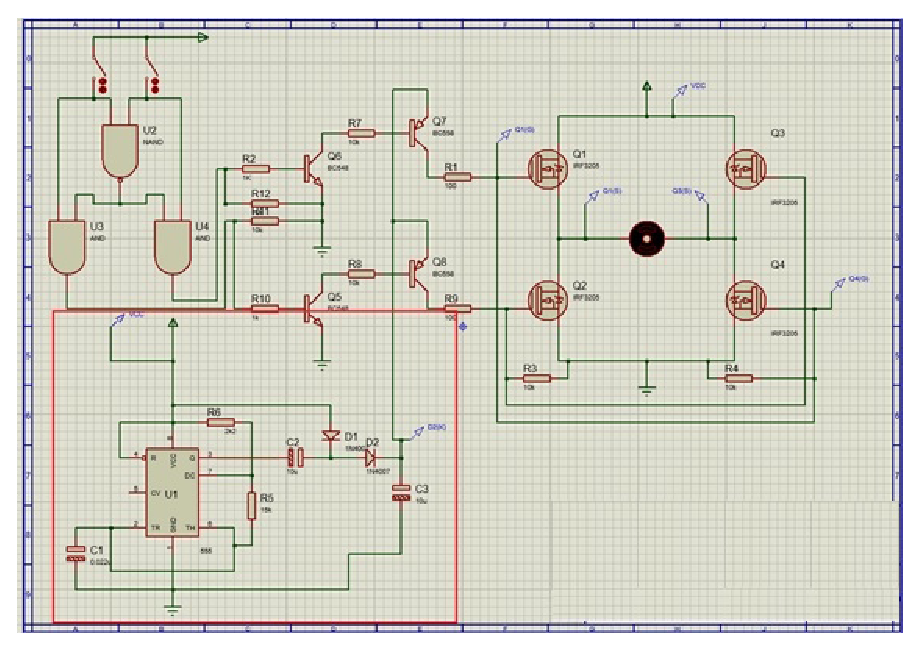
\includegraphics[keepaspectratio=true,scale=0.8]{figuras/referencialteorico/figurax_4.eps}
	\caption{Circuito elevador te tensão}
	\label{fig:figx+4}
\end{figure}


Para facilitar e proteger o sistema, será construído um distribuidor que vai ser basicamente uma placa que facilitará a conexão de todos os outros módulos ao sistema, assim não será necessário que haja reduções de tensão tão drásticas nos módulos, pois essa já estará pronta no distribuidor.

O distribuidor vai ser responsável por alimentar os motores elétricos e os módulos de controle dos movimentos da cadeira de rodas. Ele contará com um bloco de entrada que estará conectado diretamente nos terminais da bateria, onde a partir desse bloco de entrada teremos duas saídas de distribuição, uma com 12 volts e outra com 5 volts.

A saída de distribuição de 12 volts será realizada através de cabos que serão conectados nos terminais dos motores. Essa saída será dupla, ou seja, cada motor terá sua alimentação individual, sendo que para proteção dos dois motores, utilizaremos fuzíveis inseridos antes dos plugs dos moteres, para que caso ocorra alguma variação de corrente, os motores não sejam danificados.

A saída de distribuição de 5 volts será proveniente da utilização de um regulador de tensão 7805. Serão utilizados diodos zeners(falar qual) que garantirão que a tensão se mantenha estável nos 5 volts. Essa saída será responsável pela alimentação das duas pontes H, da Raspberry Pi, dos 3 msp430 e do joystick.

Esse distribuidor de tensão pode ser visto no diagrama apresentado na figura \ref{fig:diagrama_controle}.

\begin{figure}[!htb]
	\centering
	\includegraphics[keepaspectratio=true,scale=0.4]{figuras/resultados/fluxograma}
	\caption{Diagrama do sistema de controle}
	\label{fig:diagrama_controle}
\end{figure}

\subsection{Funcionamento e Estratégia de Uso}

\textbf{Joystick - Microcontroladores}

Em relação aos microcontroladores utilizados para transmitir as informações do "joystick" até o motor, serão utilizados 2 MSPs e 1 Raspberry Pi.

\begin{enumerate}
  \item O MSP do "Joystick" tem a função de receber o sinal analógico do "Joystick", transformá-lo em digital e enviá-lo para o Raspberry Pi. A rotina de conversão e transmissão dos dados referentes ao “Joystick” é controlada via TimerA, o principal temporizador do MSP utilizado, este temporizador gera uma interrupção a uma taxa de amostragem definida. A cada interrupção, o MSP lê as entradas analógicas referentes ao “Joystick” e as converte em valores digitais de um byte utilizando do SAR ADC (Successive Approximation ADC) interno ao MSP, em seguida estas informações são enviadas para o Raspberry Pi via serial, utilizando o protocolo UART (Universal Asynchronous Receiver/Transmitter), antecedidas de um cabeçalho definido, este cabeçalho é essencial para uma correta leitura dos dados pelo Raspberry Pi.
  \item O Raspberry Pi tem a função de  receber estes dados via UART. Este recebimento é controlado via interrupção, com a intenção de não onerar a "thread"principal do programa. Ao se receber esta informação, então é feita a tradução dos valores para intensidade e direção de cada motor. Após esta tradução os dados são enviados, via UART, para o MSP dos motores.
  \item O MSP dos motores tem a função de receber os dados traduzidos do Raspberry Pi para os motores, utilizando como intermediário uma Ponte-H para cada motor. O MSP ao receber as informações via UART, consegue gerar 2 ondas quadradas, uma para cada motor, a serem transmitidas via Ponte H.
\end{enumerate}

\textbf{Joystick - Desenvolvimento em Placa}

Foram feitas algumas tentativas para o desenvolvimento do Joystick com a confecção de uma placa de circuito impresso, porém devido a organização dos pinos não foi possível finalizar a mesma. Foi comprado um Joystick que possui cinco pinos, sendo um para alimentação 5V, outro para GND, dois para as direções, vertical e horizontal e ainda outro para um botão, conforme pode ser visto na figura \ref{joy}.

\begin{figure}[!htb]
	\centering
	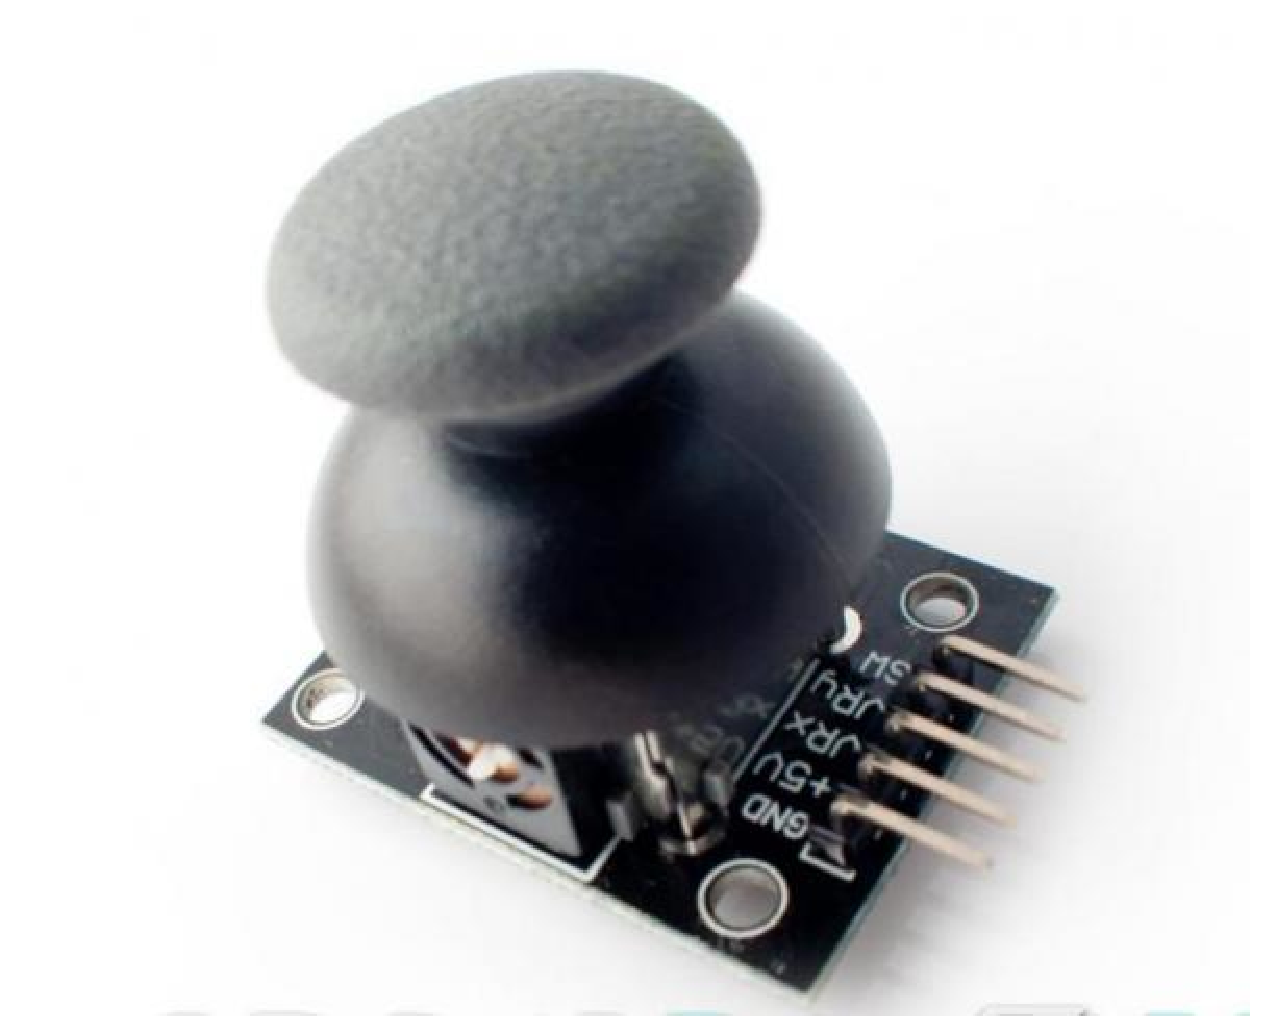
\includegraphics[keepaspectratio=true,scale=0.5]{figuras/referencialteorico/joy.eps}
	\caption{Joystick de cinco pinos}
	\label{joy}
\end{figure}

O usuário terá acesso ao Joystick e ainda a dois painéis simples, um deles vai indicar a velocidade do sistema e o outro para mostrar o nível da bateria. Os medidores de bateria e velocidade, serão indicados por LEDs que mostrarão o nível que o sistema se encontra e serão posicionados de forma que facilite a vida do usuário.

\textbf{Joystick - Conversão dos Valores}

A estratégia de conversão dos potênciometros em intensidade para os motores é feita da seguinte forma:

1. Mapeamento dos valores dos potênciometros em estados conforme figura \ref{tab:tabela-pots}.

\begin{table}[!ht]
\centering
\resizebox{\textwidth}{!}{%
\begin{tabular}{|c|c|c|}
\hline
Valor Potenciômetro 1 (motor1) & Valor Potenciômetro 2 (motor2) & Estado \\ \hline
255 & 255 & Para frente \\ \hline
255 & 0 & Virar para direita (próprio eixo) \\ \hline
255 & 127 & Virar para direita (eixo motor 2) frontal \\ \hline
127 & 127 & Parado \\ \hline
127 & 255 & virar para esquerda (eixo motor 1) frontal \\ \hline
127 & 0 & virar para esquerda (eixo motor 1) traseiro \\ \hline
0 & 0 & Para trás \\ \hline
0 & 255 & Virar para esquerda (próprio eixo) \\ \hline
0 & 127 & virar para direita (eixo motor 2) traseiro \\ \hline
\end{tabular}
}
\caption{Mapeamento dos valores conforme estado}
\label{tab:tabela-pots}
\end{table}

2. Conforme o estado mapeado, a intensidade e direção do motor podem ser definidas conforme figura \ref{tab:tabela-pots2}.

\begin{table}[!ht]
\centering
\resizebox{\textwidth}{!}{%
\begin{tabular}{|c|c|c|}
\hline
Estado                                      & Motor 1(Intensidade(\%), Direção) & Motor 2(Intensidade (\%), Direção) \\ \hline
Para frente                                 & (100, + )                         & (100, + )                          \\ \hline
Virar para direita (próprio eixo)           & (100, +)                          & (100, -)                           \\ \hline
Virar para direita (eixo motor 2) frontal   & (100, +)                          & (0 , *)                            \\ \hline
Parado                                      & (0, *)                            & (0, *)                             \\ \hline
virar para esquerda (eixo motor 1) frontal  & (0, *)                            & (100, +)                           \\ \hline
virar para esquerda (eixo motor 1) traseiro & (0, *)                            & (100, -)                           \\ \hline
Para trás                                   & (100, -)                          & (100, -)                           \\ \hline
Virar para esquerda (próprio eixo)          & (100, -)                          & (100, +)                           \\ \hline
\end{tabular}
}
\caption{Intesidade e direção dos motores conforme estado. Asteriscos simbolizam motor sem direção}
\label{tab:tabela-pots2}
\end{table}

Para facilitar e proteger o sistema, será construído um distribuidor que será, basicamente, uma placa que facilitará a conexão de todos os outros módulos ao sistema, assim não será necessário que haja reduções de tensão tão drásticas nos módulos, pois esta já estará pronta no distribuidor. O distribuidor contará ainda como um circuito de proteção para os demais periféricos.

Na parte de sensoreamento utilizaremos circuitos e sensores para indicar o nível de bateria e a velocidade da cadeira de rodas.

Para indicar o nível de bateria, serão utilizados comparadores que a partir da tensão presente na bateria, alimentem LED's vermelhos, amarelos e verdes, indicando uma escala de cores, para assim mostrar qual o nível de bateria que ainda resta no sistema.
